\section*{Assignment 07: Inequality and Responsibility}
\addcontentsline{toc}{section}{Assignment 07: Inequality and Responsibility}

\subsection*{Diagnosing inequality risks}
I drew directly on Lecture~8's inequality checklist \citep{Lecture08}. Resource light NGOs fear hidden costs and lack staff to manage another platform, while humanities and design faculties often see their work sidelined because evaluation rubrics prioritise business style outputs. \citet{Srnicek2017} and \citet{Choudary2016} both warn that governance must match participant value logic, otherwise network effects amplify inequity. Those insights shape the interventions here.

\subsection*{Targeted interventions with evidence}
\begin{itemize}
  \item \textbf{Resource light NGOs.} I package a lean onboarding kit: templated briefs, an auto generated progress report, and a buddy system where experienced students shadow the first sprint. The VirtuAI case showed how social onboarding offsets scarce staff, so this kit directly applies that lesson \citep{Gunasilan2024}.
  \item \textbf{Humanities and design faculties.} Faculty sandboxes let departments define success metrics beyond revenue, including qualitative reflection and cultural impact. The sandbox also supports offline uploads for analogue prototypes. This follows \citet{Reillier2017}'s guidance on modular governance so each segment keeps legitimacy.
  \item \textbf{Cross campus community.} A fairness clause tracks hours contributed versus fees paid and unlocks waivers once volunteer time passes a threshold. An inclusion council with representatives from every faculty and NGO cluster reviews data policy changes quarterly. Finally, an impact audit inspired by the DineTogether case checks whether new features skew toward well funded actors \citep{Rennella2023}.
\end{itemize}

\subsection*{Operationalising fairness}
To execute these ideas I outlined concrete artefacts. The onboarding kit lives in a shared Notion space with checklists, video walkthroughs, and a budget calculator. Faculty sandboxes launch as private workspaces seeded with templates for qualitative assessment. The fairness clause appears inside the terms of use with a simple formula: if an organisation contributes more than thirty unpaid hours in a quarter, transaction fees drop by half for the next two briefs. Inclusion council meetings follow an agenda based on \citet{Lecture11}'s discussion of legitimacy: review metrics, approve policy changes, hear community concerns.

The messaging system in Figure~\ref{fig:chat-system} ties everything together. Dedicated channels route accessibility requests, translation help, and fairness feedback. Moderators use templated responses that link back to the clause so tone stays consistent while still allowing personal empathy. This design treats communication as infrastructure, echoing \citet{Choudary2016}'s advice to nurture community level interactions.

\begin{figure}[H]
  \centering
  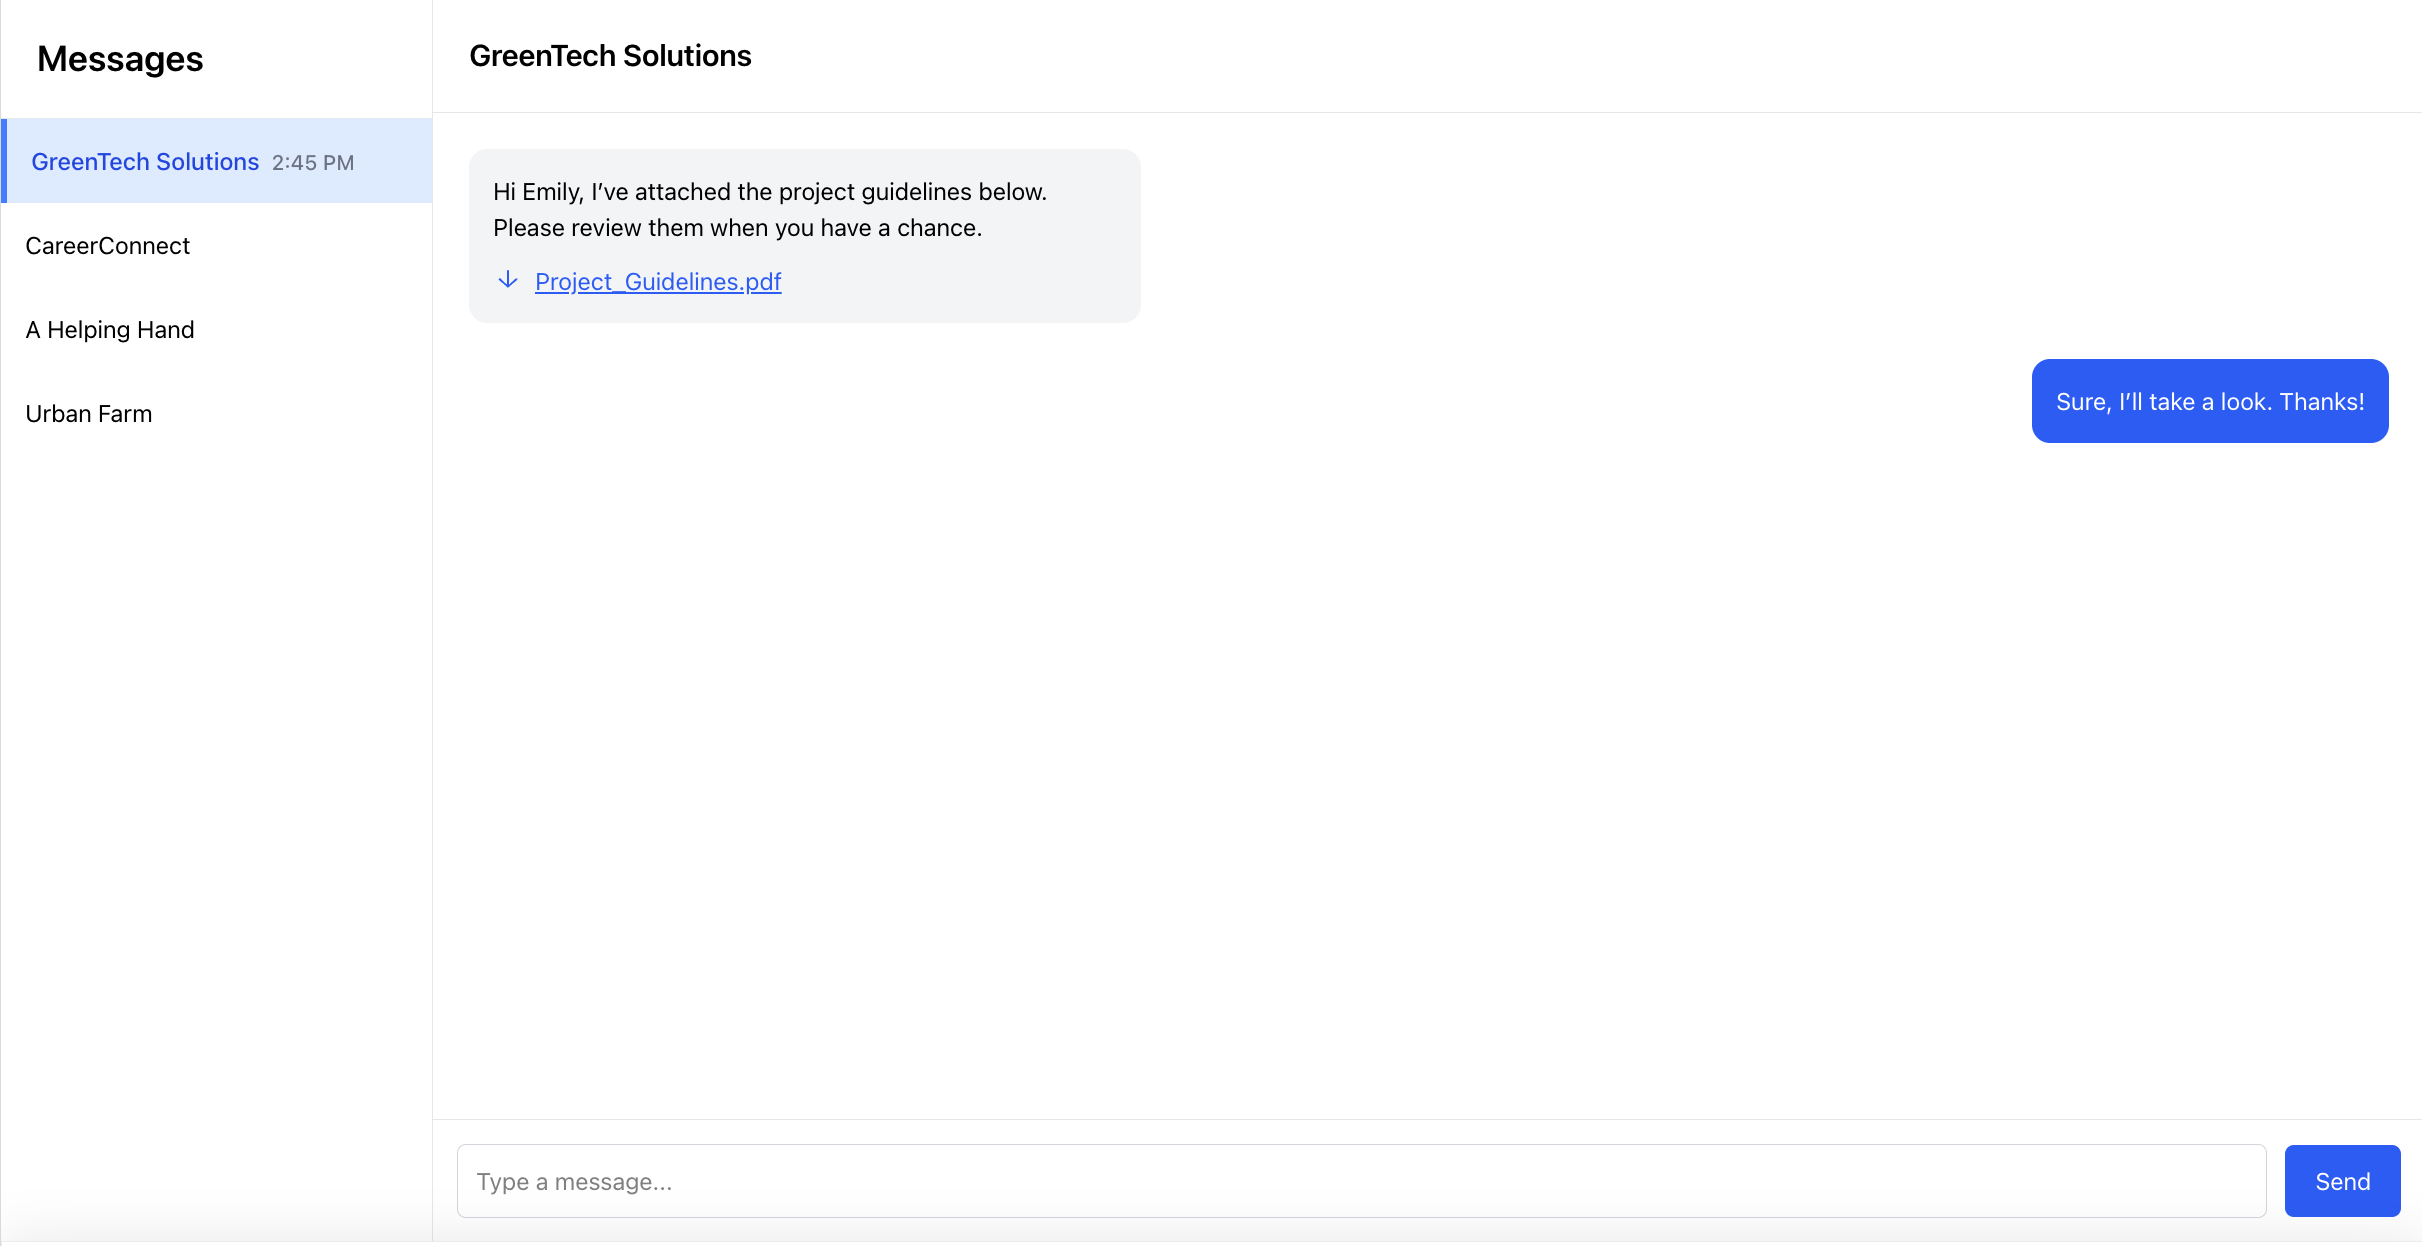
\includegraphics[width=0.85\linewidth]{figures/Messengersystem.png}
  \caption{Messaging workspace mock up coordinating inclusion support.}
  \label{fig:chat-system}
\end{figure}

To redistribute opportunities I also sketched a mutual aid pool. Partners with surplus capacity can pledge design time, translation support, or data analysis hours. The pool uses a simple ledger system managed by the inclusion council. Participants earn recognition badges when they contribute and can request help through the chat interface. Lecture~9 emphasised that platforms should enable peer to peer support, and this pool operationalises that advice \citep{Lecture09}. Continuous reporting on usage keeps the promise credible.
